%%%%%%%%%%%%%%%%%%%%%%%%%%%%%%%%%%%%%%%%%%%%%%%%%%%%%%%%%%%%%%%%%%%%%%
% LaTeX Template: Beamer arrows
%
% Source: http://www.texample.net/
% Feel free to distribute this template, but please keep the
% referal to TeXample.net.
% Date: Nov 2006
% 
%%%%%%%%%%%%%%%%%%%%%%%%%%%%%%%%%%%%%%%%%%%%%%%%%%%%%%%%%%%%%%%%%%%%%%
% How to use writeLaTeX: 
%
% You edit the source code here on the left, and the preview on the
% right shows you the result within a few seconds.
%
% Bookmark this page and share the URL with your co-authors. They can
% edit at the same time!
%
% You can upload figures, bibliographies, custom classes and
% styles using the files menu.
%
% If you're new to LaTeX, the wikibook is a great place to start:
% http://en.wikibooks.org/wiki/LaTeX
%
%%%%%%%%%%%%%%%%%%%%%%%%%%%%%%%%%%%%%%%%%%%%%%%%%%%%%%%%%%%%%%%%%%%%%%

\documentclass{beamer} %
% \usetheme{Boadilla}
\usepackage[latin1]{inputenc}
\usefonttheme{professionalfonts}
\usepackage{times}
\usepackage{tikz}
\usepackage{amsmath}
\usepackage{verbatim}
\usetikzlibrary{arrows,shapes}


\usetheme{Warsaw}

\setbeamercolor{normal text}{fg=yellow,bg=black!90}
\setbeamercolor{structure}{fg=yellow}

\setbeamercolor{alerted text}{fg=red!85!black}

\setbeamercolor{item projected}{use=item,fg=black,bg=item.fg!35}

\setbeamercolor*{palette primary}{use=structure,fg=structure.fg}
\setbeamercolor*{palette secondary}{use=structure,fg=structure.fg!95!black}
\setbeamercolor*{palette tertiary}{use=structure,fg=structure.fg!90!black}
\setbeamercolor*{palette quaternary}{use=structure,fg=structure.fg!95!black,bg=black!80}

\setbeamercolor*{framesubtitle}{fg=green}

\setbeamercolor*{block title}{parent=structure,bg=black!60}
\setbeamercolor*{block body}{fg=black,bg=black!10}
\setbeamercolor*{block title alerted}{parent=alerted text,bg=black!15}
\setbeamercolor*{block title example}{parent=example text,bg=black!15}

\useoutertheme{split}
\setbeamertemplate{navigation symbols}{}

\title{Membrane-localized Keratin-14 \\ promotes invasion}
\author{Yohanes Tsehay \\ \& Andrei Kucharavy}
%\title{Spectral Analysis}
\institute{Joel Bader's Lab}
\date{10/04/2018}
%\logo{
\includegraphics[height=1.5cm]{hopkinslogo.jpg}}
%\logo{
\includegraphics[height=1.5cm]{ctd2_overall.png}}
\titlegraphic{%
   
\includegraphics[width=5cm]{Hopkins_logo_2.png}\hspace*{2.75cm}~%
   
\includegraphics[width=3cm]{ctd2_overall.png}\hspace*{1.75cm}%
   }


\begin{document}

\tikzstyle{every picture}+=[remember picture]

\everymath{\displaystyle}

\frame{\titlepage}

\begin{frame}
\frametitle{Overview}

\begin{itemize}
		% \item Background Information
		\item Objective
		\item Methods
		\item Results
		\item Discussion
		\item Future Directions
\end{itemize}

\end{frame}


% \begin{frame}
% \frametitle{Background}

% \begin{itemize}
% 		\item Metastasis is one of the main determinants of patient prognosis 
% 		\item Mortality is often due to systemic spread of tumor and not in situ proliferation
% 		\begin {Example}
%		5-year survival rate for invasive breast cancer at diagnosis is:
%		\begin {itemize}
%	\item 99\% for patient with \alert{local tumors}
%	\item 85\% for patients with \alert{regional spread}
%	\item 26\% for those with \alert{tumors that have spread to distance organs} \cite{tarver2012cancer}
%		\end {itemize}
%		\end {Example}
%		\item Currently, the molecular mechanism of metastasis is not well understood
%		\item Neoplastic drug interventions mostly target proliferation, not metastatic transformation
%\end{itemize}

% \end{frame}

\begin{frame}
	\frametitle{Quantifying the Invasive Potential of Tumors}
	\begin{itemize}
		\item Why would we need to make a system that quantifies the invasive potential of tumors?
		\begin{itemize}
				\item Quantitative phenotypes are more amenable to systemic analysis
				\item They can be used in population genetics methods, where genetic variations and invasive potential of tumors can be studied by directly perturbing candidate genes
				\item Such studies can lead to the discovery of new drugs for cancer therapy which can ultimately have a positive impact on the poor prognosis seen in patients with metastatic carcinoma 		\end{itemize}
	\end{itemize}
\end{frame}


\begin{frame}
	\frametitle{Phenotype quantification allows us to pull out the molecular correlates}
	\begin{itemize}
		\item Invasivenes quantification allows us to calculate the genetic contribution of individual genes
		\begin{itemize}
				\item Quantitive characterization allows us to detect even minor contributors
				\item Quantification of phenotype allows us to calculate the interaction between different genes
				\item The fine-grainness of the quantification allows us to perform genetic correlation at the genome scale
		\end{itemize}
	\end{itemize}
\end{frame}


\begin{frame}
	\frametitle{Why we use Keratin 14 as a proof of expression?}
	\begin{itemize}
			\item Keratin 14 is a know biomolecular marker for metastasis
			\item {[Shamir .. Bader Ewald 2014]} challenge the epithelial-to-mesenchymal transition requirement for metastasis, and instead, provide evidence in support of a model based on Twist1 induced dissemination of cytokeratin positive epithelial cells
			\item {[Cheung .. Bader Ewald 2016]} demonstrated that tumor cells only can invade and metastasize in clusters
			\item in the same paper, Cheung et al. suggested Keratin 14-associated pathways are key regulators of metastasis
	\end{itemize}
\end{frame}


\begin{frame}
	\frametitle{Project Objective}
	\begin{itemize}
		\item We will test whether K14 is correlated with invasiveness:
		\begin{enumerate}
			\item Total K14 
			\item Peripheral K14
			\item Central K14
		\end{enumerate}
	\end{itemize}
\end{frame}


\begin{frame}
	\frametitle{Our Data}
	\begin{itemize}
			\item MMTV-PyMT transgenic mice were be used to produce a supply of organoids
			\item Tumors were removed from 4 mice and a total of 90 - 150 small and large organoids were generated per tumor ($\approx$ 300 organoids in total per tumor)
			\item The organoids were imaged using differential interference contrast (DIC) microscopy
			\item The images were manually traced using \textsc{ImageJ} to define organoid boundaries
			\item corresponding K14 images are available
	\end{itemize}
\end{frame}

% \begin{frame}
% 	\frametitle{Our Computer Model (Spectral Power)}
%	\begin{itemize}
%		\item the manually traced boundary is defined by a pair of points \(\{x_v, y_v\}\) for $p \in [0, P-1]$, where $P$ is the total number of points
%		\item First the overall length $L$ was calculated
%		\item $L = \sum_{v=1}^{V-1} \sqrt{(x_v - x_{v-1})^2 + (y_v - y_{v-1})^2}$
%		\item Next, an equally spaced grid was defined with distance $L/M$ between adjacent points, where $M=128$
%		\item Then, linear interpolation was used to generate a new boundary with equally spaced points \(\{x_j, y_j\}\), where $j \in \{0,1,...,M-1\}$  
%	\end{itemize}
% \end{frame}

%\begin{frame}
%	\frametitle{Fourier Transform of the edge shape}
%	\begin{itemize}
%			\item Then, a fast Fourier transform on the newly generated boundary is performed according to:
%			\newline
%			$\hat{x}_k = \sum_{j=0}^{M-1} e^{-2\pi ijk/M} x_j$ 
%			\newline
%			$\hat{y}_k = \sum_{j=0}^{M-1} e^{-2\pi ijk/M} y_j$ 
%			\item where $k \in \{0,1,...,M/2+1\}$
%	\end{itemize}
%\end{frame}

\begin{frame}
	\frametitle{Fourier Transform reminder}
	\begin{figure}
		\centering
		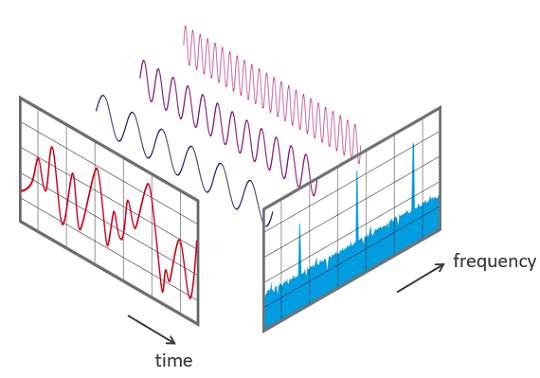
\includegraphics[width=7cm]{FFT-Time-Frequency-View.png}
	\end{figure}
\end{frame}


% \begin{frame}
%	\frametitle{Spectral Power}
%	\begin{itemize}
%			\item The spectral power $P_k$ is given by:
%			\newline
%			$P_k = |\hat{x}_k|^2 + |\hat{y}_k|^2$
%			\newline
%			\item where $k \in \{0,1,...,M/2+1\}$
%			\item $P_0$ is the center and $P_1$ is used to normalize the total power given by:
%			\newline
%			$P_{total} = \sum_{k=2}^{M/2+1} P_k/P_1$
%			\item this produces a spectral power that is scale invariant in addition to being transilation and rotation invariant. 
%			\item we use a slightly more comples formula to smooth out the artifacts:
%			\newline
%			$w \equiv \sum_{k=2}^{M/2} (M/\pi)^2 \sin^2(\pi k/M) \cos^2(\pi k/M) P_k/P_1$
%	\end{itemize}
% \end{frame}

%\begin{frame}
%	\begin{itemize}
%			\item Means and parametric derivative transforms are estimated
%			\item This is done to smooth out artifacts in the boundary 
%			\item The transform for $\bar{x}_{j\prime} \equiv (x_{j\prime+1/2} + x_{j\prime-1/2})/2$ is: 
%			\newline
%			$\hat{\bar{x}}_k = \cos(\pi k/M)\hat{x}$ 
%			\newline
%			\item The transform for $\dot{x}$ is: 
%			\newline
%			$\hat{\dot{x}} = (iM/\pi)\sin(\pi k/M)\hat{x}$
%			\item Therefore, the final weighted spectral power becomes:
%			\newline
%			$w \equiv \sum_{k=2}^{M/2} (M/\pi)^2 \sin^2(\pi k/M) \cos^2(\pi k/M) P_k/P_1$
%	\end{itemize}
%\end{frame}

\begin{frame}
	\frametitle{Example}
	\begin{figure}
		\centering
		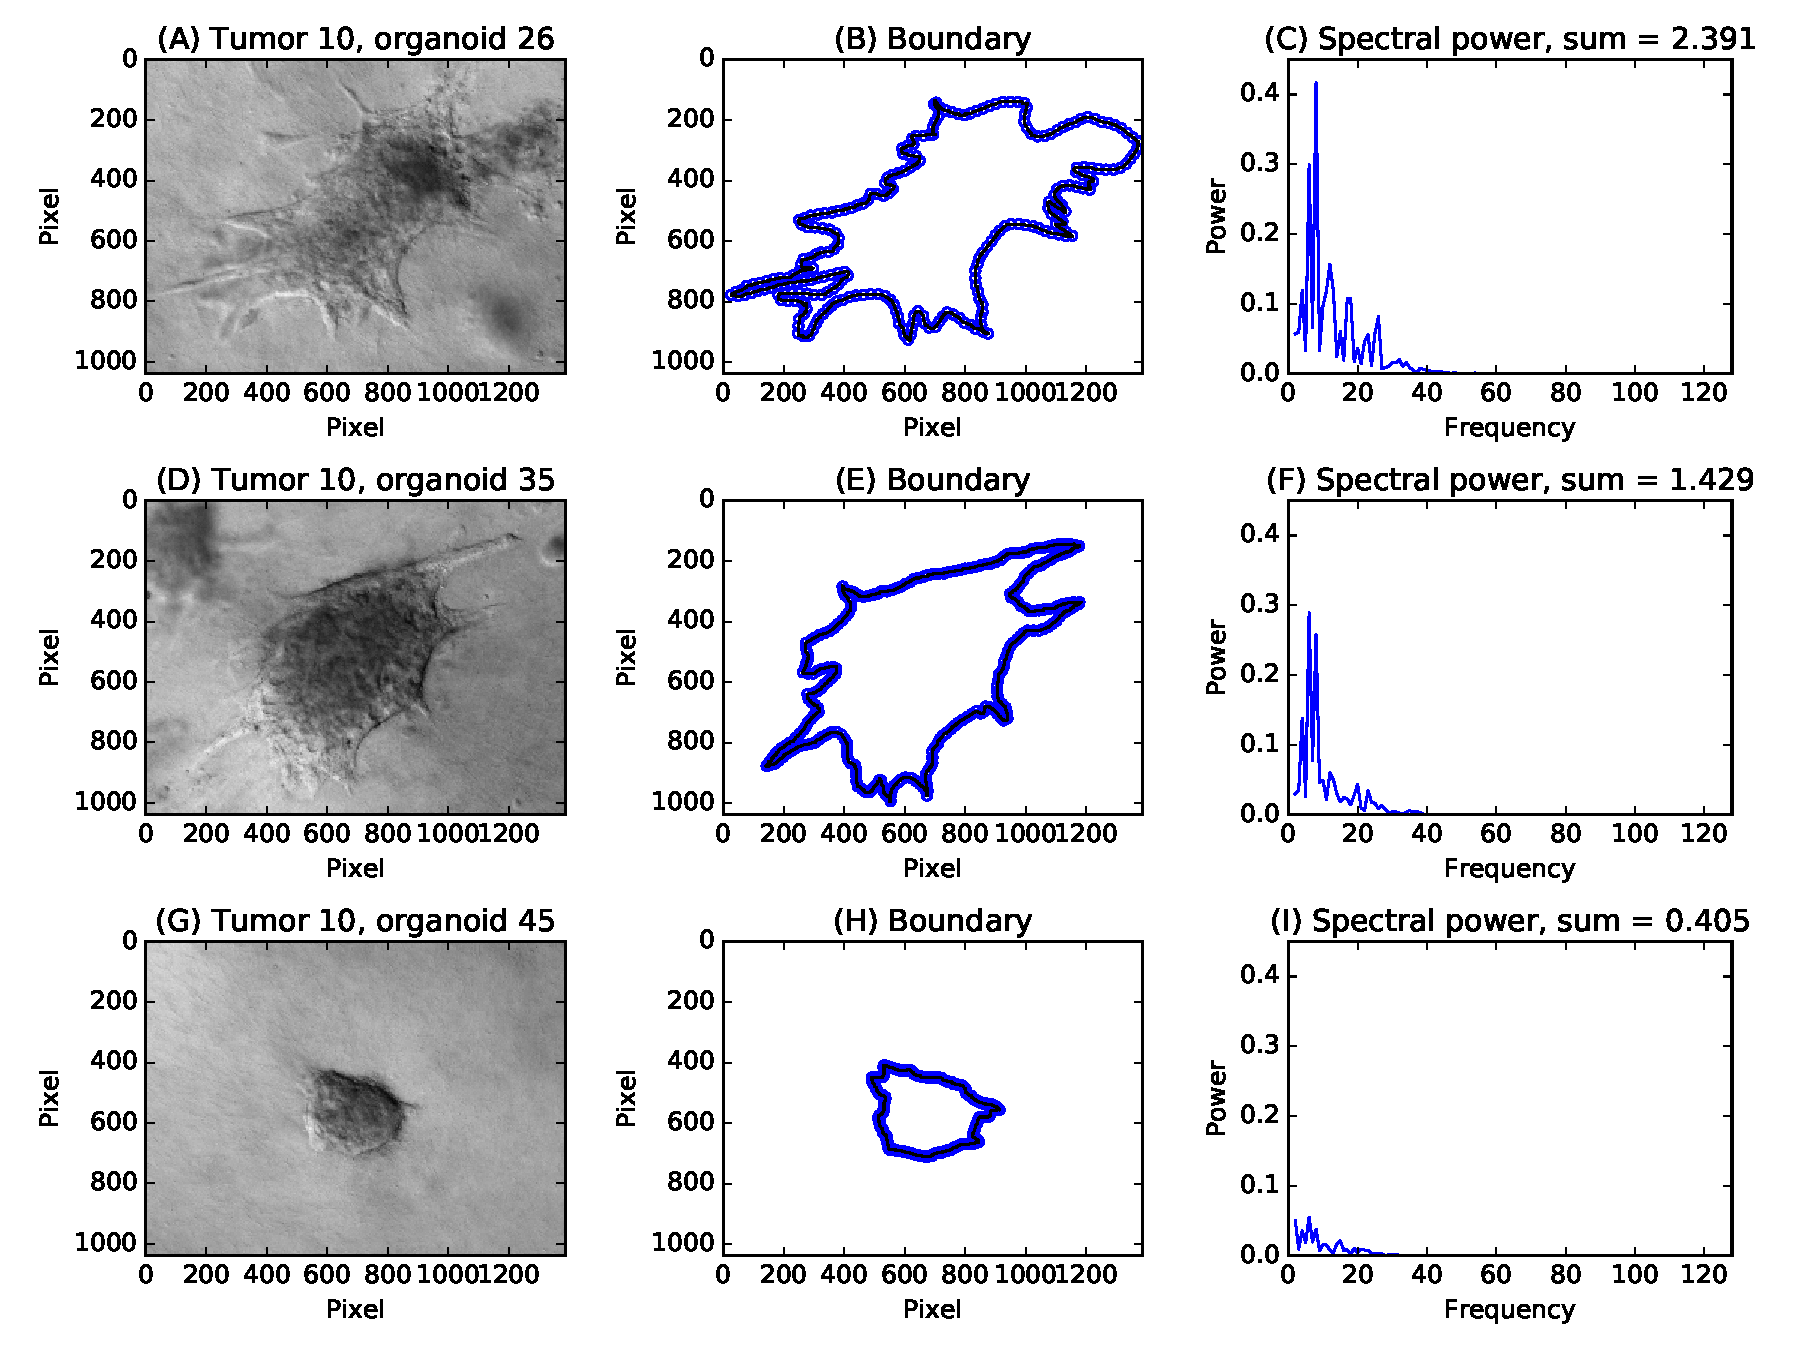
\includegraphics[height=8cm]{fig1_CTN010.pdf}
	\end{figure}
\end{frame}

\begin{frame}
	\frametitle{Analysis}
	\begin{itemize}
			\item Features that we considered to compare against our model include the following:
			\begin{itemize}
					\item Fractional area of the organoid 
					\item K14 Mean
					\item K14 Sum of pixels intensities in the periphery
					\item K14 Sum of pixels intensities in the center
					\item K14 total pixel intensity sum 
			\end{itemize}
	\end{itemize}
\end{frame}

\begin{frame}
	\frametitle{An Efficient Way to Get Peripheral Pixels}
	\begin{enumerate}
			\item Generate a mask from the boundary
			\item make a disk to be used as a kernel with which to convolve the mask
			\begin{Example}
				A disk with a radius of 3 is:
				\newline
				$k = \begin{bmatrix}
					0 & 0 & 0 & 1 & 0 & 0 & 0 \\
					0 & 1 & 1 & 1 & 1 & 1 & 0 \\
					0 & 1 & 1 & 1 & 1 & 1 & 0 \\
					1 & 1 & 1 & 1 & 1 & 1 & 1 \\
					0 & 1 & 1 & 1 & 1 & 1 & 0 \\
					0 & 1 & 1 & 1 & 1 & 1 & 0 \\
					0 & 0 & 0 & 1 & 0 & 0 & 0
				\end{bmatrix}$
			\end{Example}
	\end{enumerate}
\end{frame}

\begin{frame}
	
		\frametitle{Convolution}
\begin{description}
	\item	
	\begin{figure}	
		\centering
		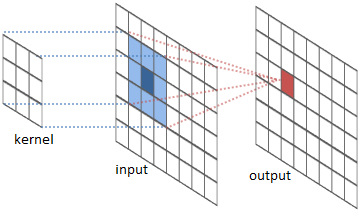
\includegraphics[height=4cm]{RiverTrain-ImageConvDiagram}  \hspace*{4cm}
	\end{figure}
	\item $ (f*g)[i, j] = \sum_{k=minW_{kernel}}^{maxW_{kernel}}\sum_{l=minH_{kernel}}^{maxH_{kernel}} f[i-k, j-l]g[k, l] $
\end{description}
\end{frame}

\begin{frame}
	\frametitle{Convolution for efficient organoid segmentation}
	\begin{figure}
		\centering
		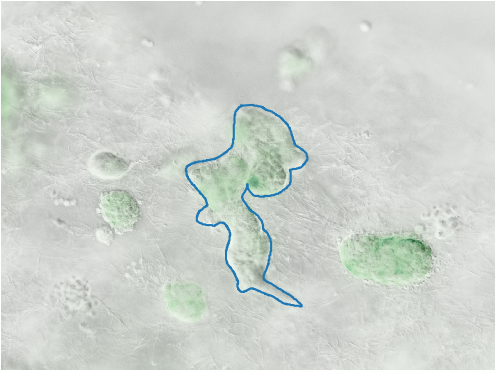
\includegraphics[width=5cm]{Border}
		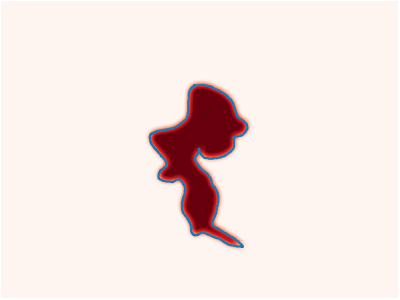
\includegraphics[width=5cm]{convolved_array}
		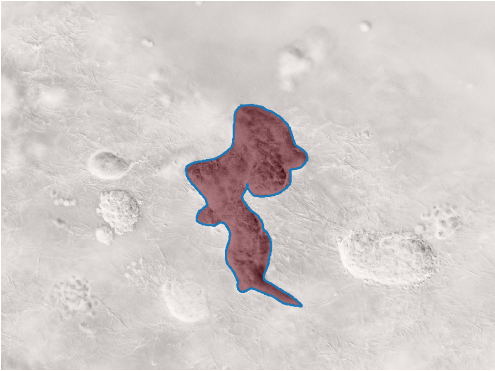
\includegraphics[width=3.5cm]{internal_map}
		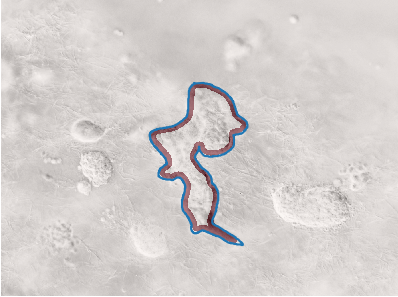
\includegraphics[width=3.5cm]{inner_border}
		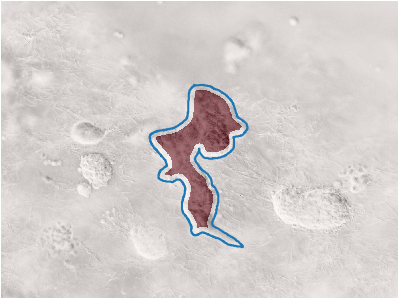
\includegraphics[width=3.5cm]{internal_area}
		\begin{columns}
		\column{0.5\textwidth}
			radius, $r= 20$ pixel size $\sim 0.5 \mu$ 
		\end{columns}
	\end{figure}
\end{frame}

\begin{frame}
	\frametitle{Peripheral K14 expression correlates with invasive potential}
	\begin{figure}		
		\centering
		%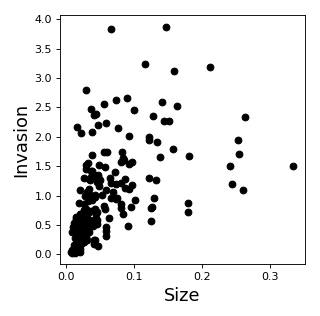
\includegraphics[width=4cm]{Corr_size}
		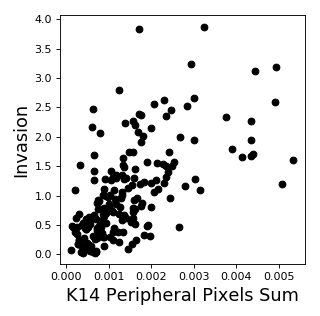
\includegraphics[height=5cm]{Corr_K14}
		%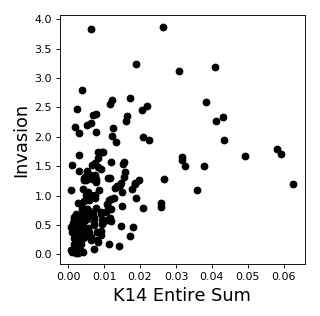
\includegraphics[width=4cm]{Corr_K14_central}
		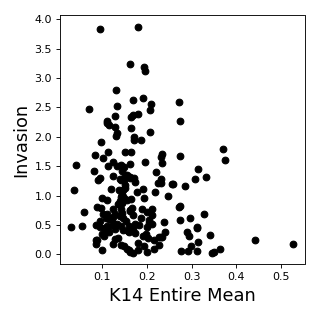
\includegraphics[height=5cm]{Corr_K14_mean}
	\end{figure}
\end{frame}


\begin{frame}
	\begin{figure}
		\frametitle{Peripheral K14 explains correlates with invasive potential the best}
		\centering
		\resizebox{\textwidth}{!}{
		 \begin{tabular}{||c c c c||}
			\hline
			 & \multicolumn{3}{|c|}{$r^2$ by mouse} \\
			 \hline
			 Organoids (mouse\#) & 1 & 2 & 3  \\ [0.5ex]
			 \hline\hline
			  \textbf{Peripheral sum K14} & \textbf{0.39} & \textbf{0.43} & \textbf{0.29} \\
			 \hline
			 Centeral sum K14 & 0.21 & 0.19 & 0.11 \\
			 \hline
			 Entire sum K14 & 0.22 & 0.22 & 0.12 \\
			 \hline
%			 K14 Mean & 0.02 & 0.04 & 0.03 \\ [1ex]
%			 \hline
			Size & 0.27 & 0.33 & 0.27 \\
			 \hline
		\end{tabular}
		}
	\end{figure}
\end{frame}

\begin{frame}
	\frametitle{Discussion}
	\begin{itemize}
			\item Looking at K14 expression in the periphery of the organoids is promising
			\item K14 expression in the center of the organoids correlates less with spectral score than peripheral K14 expression 
			\item K14 Mean doesn't seem to contribute much
			\item Using peripheral K14 expression seems to have more significance for large organoids 
			\item Fractional area and peripheral K14 expression give comparable $r^2$ values
	\end{itemize}
\end{frame}

\begin{frame}
	\frametitle{Future Directions}
	\begin{itemize}
			% \item Mouse \#4 data seems to be slightly off, so fix it
			% \item Establish statistical significance for our hypothesis 
			\item Apply our model on human organoids generated from breast tumors 
			\newline
	\end{itemize}
\end{frame}


\begin{frame}
 	\frametitle{Thank you!}
	\begin{itemize}
			% \item Mouse \#4 data seems to be slightly off, so fix it
			% \item Establish statistical significance for our hypothesis 
			\item Joel Bader
			\item Joel Bader lab members
			\newline
			\item Andrew Ewald
			\item Veena Padamanaban (data)
			\item Andrew Ewald members
			\newline
			\item Cancer Target Discovery and Development 
	\end{itemize}
\end{frame}

%%%%%%%%%%%%%%%%%%%%%%%%%%%%%%%%%%%%%%%%%%%%%%%%%%%%%%%%%%%%%%%%%%%%%%%%%%%%

%\begin{frame}
%\frametitle{Template}
%
%\tikzstyle{na} = [baseline=-.5ex]
%
%\begin{itemize}[<+-| alert@+>]
%    \item Coriolis acceleration
%        \tikz[na] \node[coordinate] (n1) {};
%\end{itemize}
%
%% Below we mix an ordinary equation with TikZ nodes. Note that we have to
%% adjust the baseline of the nodes to get proper alignment with the rest of
%% the equation.
%\begin{equation*}
%\vec{a}_p = \vec{a}_o+\frac{{}^bd^2}{dt^2}\vec{r} +
%        \tikz[baseline]{
%            \node[fill=blue!20,anchor=base] (t1)
%            {$ 2\vec{\omega}_{ib}\times\frac{{}^bd}{dt}\vec{r}$};
%        } +
%        \tikz[baseline]{
%            \node[fill=red!20, ellipse,anchor=base] (t2)
%            {$\vec{\alpha}_{ib}\times\vec{r}$};
%        } +
%        \tikz[baseline]{
%            \node[fill=green!20,anchor=base] (t3)
%            {$\vec{\omega}_{ib}\times(\vec{\omega}_{ib}\times\vec{r})$};
%        }
%\end{equation*}
%
%\begin{itemize}[<+-| alert@+>]
%    \item Transversal acceleration
%        \tikz[na]\node [coordinate] (n2) {};
%    \item Centripetal acceleration
%        \tikz[na]\node [coordinate] (n3) {};
%\end{itemize}
%
%% Now it's time to draw some edges between the global nodes. Note that we
%% have to apply the 'overlay' style.
%\begin{tikzpicture}[overlay]
%        \path[->]<1-> (n1) edge [bend left] (t1);
%        \path[->]<2-> (n2) edge [bend right] (t2);
%        \path[->]<3-> (n3) edge [out=0, in=-90] (t3);
%\end{tikzpicture}
%\end{frame}

% \bibliography{refs}
% \bibliographystyle{apalike}

\end{document}
